\documentclass[conference]{IEEEtran}
\usepackage{fontspec}
\setmainfont[Path=C:/Windows/Fonts/]{NotoSansSC-VF.ttf}
\XeTeXlinebreaklocale "zh"
\XeTeXlinebreakskip = 0pt plus 1pt
\usepackage{amsmath,amssymb}
\usepackage{booktabs,multirow,graphicx}
\usepackage{xcolor,url}
\title{跨轨道剩余寿命预测的仅源域路线选择：经审计的时序 TCN 研究}
\author{BRPHM Research Group}
\begin{document}
\sloppy
\maketitle

\begin{abstract}
跨轨道剩余寿命（RUL）预测会受到归一化、时序表示、损失函数和后处理的细小但重要的影响。本文报告一个仅使用源域的研究：在三个运行轨道（LEO500、LEO550 和 LEO700）上评估 BAT 与 RWA 两个已登记部件。研究冻结了分段 HGB/MLP 参考实现，执行六个有向源域迁移、三个残差 KS 检查，并使用六折外层晋级规则。候选选择从不读取外层标签。我们依次评估 unit-first 相对时序卷积网络（TCN）、源域拟合残差中心化、L1 变体、最差方向路线选择以及 alpha 下限约束。最终晋级候选使用源域标准化遥测、每个 unit 的最早窗口相对轨迹、三个固定随机种子的 SmoothL1 集成，以及统一的目标轨道 alpha 下限 $10^{-5}$。在六个外层折上，RMSE 与 MAE 均不劣于冻结参考：BAT 的 RMSE 差值分别为 $-3.66\times10^{-6}$、$-9.59\times10^{-6}$ 和 $-3.01\times10^{-5}$；RWA 的差值为 $-2.52\times10^{-5}$、$-1.33\times10^{-8}$ 和 $-2.94\times10^{-8}$。该结果是受控的未见轨道结果，不是总体范围或真实世界泛化结论。所有 receipt、哈希、失败路线和仅源域约束均随本文发布。
\end{abstract}
\begin{IEEEkeywords}
剩余寿命，域偏移，时序卷积网络，仅源域验证，可复现性，形式化评估
\end{IEEEkeywords}

\section{引言}
RUL 预测通常假设训练观测和测试观测服从稳定的数据生成过程。在工业遥测中，运行轨道、负载和采集条件可能改变轨迹与剩余寿命之间的关系。因此，一个模型可能改善平均验证分数，却在某个具体迁移方向上退化。当路线选择、校准和外层评估混在一起时，这种失败尤其难以发现。

本文给出 BRPHM 电化学 RUL 研究的可审计仅源域路线选择协议及其最终晋级候选。工程贡献与“提出一种普适的新域适应算法”的主张明确分开。协议冻结参考实现，使用 SHA-256 绑定每个输入张量和 receipt，评估六个有向源域迁移，检查三个残差分布，并规定只有 BAT 和 RWA 同时通过源域门禁后才能进入形式化外层评估。最终晋级规则严格要求每个 BAT/RWA 与轨道折上的 RMSE 和 MAE 都不高于冻结参考。

本研究回答三个问题：（i）unit-first 时序表示能否改善跨轨道迁移？（ii）源域拟合残差中心化和另一种损失能否修复剩余迁移失败？（iii）仅源域路线约束能否在不使用外层标签的情况下消除确定性的近参考退化？在登记的三轨道协议下，第三个问题的答案为是。但该答案不构成总体范围泛化证据；形式化证据被限定在登记轨道集合及其精确数据契约内。

\section{相关工作}
时序卷积网络在保留长感受野的同时，为循环序列模型提供了简单替代方案~\cite{bai2018tcn}。鲁棒绝对误差目标与 Huber 损失的鲁棒估计观点相关~\cite{huber1964}。域适应理论指出，迁移误差同时取决于源域误差和分布差异~\cite{ben2010domain}；本文的残差 KS 检查是工程诊断，不是泛化界。深度时序方法综述也强调，预处理和评估协议可能主导表面上的模型增益~\cite{fawaz2019review}。实现使用 PyTorch~\cite{paszke2019pytorch}，但本文不宣称这套路线选择栈是某一篇论文中的命名方法。

\section{数据与评估契约}
\subsection{登记数据}
实验使用 ModelScope 项目数据根目录中已登记的 BAT 和 RWA 张量。最终 receipt 使用的 BAT 与 RWA 时序输入均含 13 个通道，窗口长度为 30。unit 标识符中解析出三个轨道：LEO500、LEO550 和 LEO700。源域 unit 与验证 unit 按构造保持不相交。冻结参考哈希在证据包中完整记录（前后 8 位：{\scriptsize\texttt{b708df9c...fb96b6733}}）。

\subsection{指标与门禁}
对归一化目标 $y_i$ 和预测 $\hat y_i$，先按部件的 $r_{\max}$ 进行还原，再计算指标：
\begin{equation}
 \mathrm{RMSE}=\sqrt{\frac{1}{n}\sum_i(\hat y_i-y_i)^2},\qquad
 \mathrm{MAE}=\frac{1}{n}\sum_i|\hat y_i-y_i|.
\end{equation}
源域门禁在六个有向迁移上比较候选与冻结控制的指标，并使用双样本 KS 统计量比较三个无序轨道对的残差分布。候选不得出现指标或 KS 退化，并且至少有一项误差必须严格改善。形式化晋级门禁更严格，使用六个外层折（两个部件乘三个留出轨道）；每折的 RMSE 和 MAE 都必须不高于冻结参考。数值容差为 $10^{-12}$，不会为掩盖实现间的数值差异而放宽。

\begin{figure}[t]
\centering
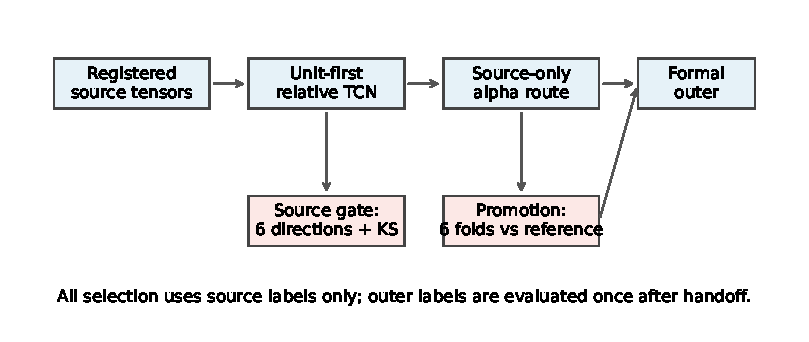
\includegraphics[width=\linewidth]{../figures/evaluation_protocol.pdf}
\caption{评估协议。路线选择和源域门禁只使用源轨道标签；交接后仅评估一次外层标签。}
\label{fig:protocol}
\end{figure}

\section{候选设计}
\subsection{Unit-first 相对表示}
对于每个窗口 $x_{u,t,:}$，先找到 unit $u$ 的最早窗口，并拼接相对基线的轨迹：
\begin{equation}
 z_{u,t,:}=\left[x_{u,t,:},\;x_{u,t,:}-x_{u,t_0,:}\right].
\end{equation}
通道均值和标准差只在源窗口上拟合。TCN 的膨胀率为 $(1,2,4)$，宽度为 16，卷积核大小为 3，dropout 为 0.05，使用 AdamW 和三个固定随机种子 $(17,42,73)$ 预测归一化 RUL。BAT 使用单调不增的保序投影；RWA 使用因果运行最小值。

\subsection{源域拟合残差中心化}
对每个训练轨道，在拟合窗口上完成预测后计算残差中位数，并乘以固定收缩因子 $s=0.25$。迁移预测前冻结修正 $-s\,\mathrm{median}(\hat y_{\mathrm{src}}-y_{\mathrm{src}})$。该修正不使用验证轨道标签。

\subsection{仅源域路线选择}
候选预测与冻结控制按照目录 $\{0,10^{-5},5\times10^{-5},\ldots,1\}^3$ 中的目标轨道 alpha 路线进行混合。最终路线对两个部件施加统一的目标轨道 alpha 下限 $10^{-5}$，随后按既有的仅源域优先级进行平局决策。按 (LEO500, LEO550, LEO700) 排列，选定路线为
\begin{align*}
\text{BAT}:&(10^{-5},10^{-5},10^{-5}),\\
\text{RWA}:&(0.02,10^{-5},10^{-5}).
\end{align*}
该下限是仅源域的数值稳定性规则，没有在外层标签上调参。

\section{失败链与实验矩阵}
研究保留失败 receipt，没有覆盖旧结果。第一个 unit-first TCN 通过两个源域门禁，但在五个形式化折上失败。加入源域拟合残差中心化后失败数降至四个；将 SmoothL1 换为加权 L1 后降至三个；最差方向源域选择进一步降至一个（RWA LEO550 的 MAE）。针对 RWA LEO550 的部件特定下限修复了该折，但 BAT 的相等性失败和 RWA LEO700 的 RMSE 仍然存在。统一下限最终修复六个折。GRU 候选未通过两个源域门禁，因此没有进入形式化评估。

\begin{table}[t]
\centering
\caption{候选矩阵。失败数是至少有一个主要指标退化的形式化折数；短横线表示不具备形式化准入资格。}
\label{tab:matrix}
\scriptsize
\begin{tabular}{lccc}
\toprule
候选 & BAT 门禁 & RWA 门禁 & 形式化失败 \\
\midrule
Unit-first TCN & 通过 & 通过 & 5\\
残差中心化 & 通过 & 通过 & 4\\
残差中心化 L1 & 通过 & 通过 & 3\\
L1 最差方向 & 通过 & 通过 & 1\\
RWA LEO550 下限 & 通过 & 通过 & 3\\
统一 alpha 下限 & 通过 & 通过 & 0\\
GRU & 失败 & 失败 & --\\
\bottomrule
\end{tabular}
\end{table}

\begin{figure}[t]
\centering
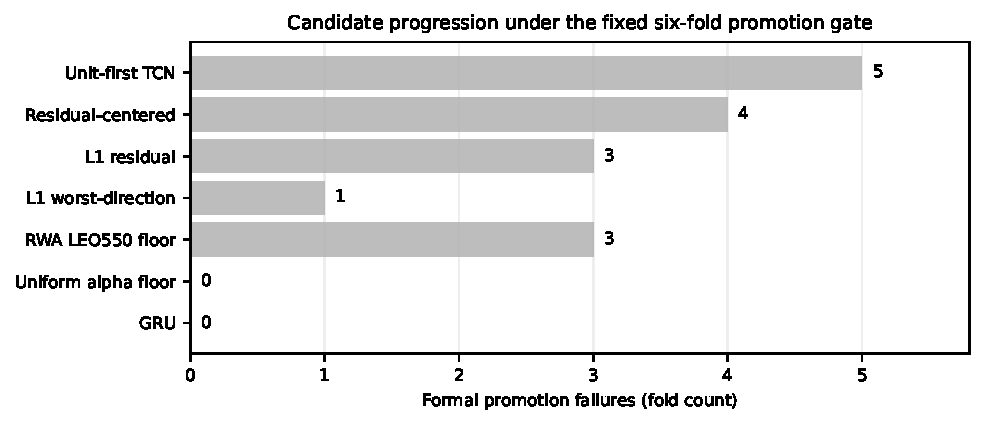
\includegraphics[width=\linewidth]{../figures/method_progression.pdf}
\caption{固定形式化门禁下的候选演进。统一 alpha 下限是该序列中第一个形式化失败数为零的候选。}
\label{fig:progression}
\end{figure}

\section{结果}
表~\ref{tab:formal} 给出最终外层折。负差值表示相对冻结参考的改善。六个折的两项差值都不为正，因此通过晋级门禁。

\begin{table*}[t]
\centering
\caption{最终晋级仅源域候选的形式化外层结果。}
\label{tab:formal}
\scriptsize
\begin{tabular}{llrrrrrr}
\toprule
部件 & 测试轨道 & 参考 RMSE & 候选 RMSE & $\Delta$RMSE & 参考 MAE & 候选 MAE & $\Delta$MAE\\
\midrule
BAT & LEO500 & 1.94580757 & 1.94580391 & $-3.66\times10^{-6}$ & 1.29659886 & 1.29659751 & $-1.35\times10^{-6}$\\
BAT & LEO550 & 1.79448883 & 1.79447924 & $-9.59\times10^{-6}$ & 1.18893968 & 1.18893575 & $-3.93\times10^{-6}$\\
BAT & LEO700 & 2.39083744 & 2.39080737 & $-3.01\times10^{-5}$ & 1.55831112 & 1.55829253 & $-1.86\times10^{-5}$\\
RWA & LEO500 & 0.02075028 & 0.02072511 & $-2.52\times10^{-5}$ & 0.01558350 & 0.01558298 & $-5.21\times10^{-7}$\\
RWA & LEO550 & 0.02027168 & 0.02027166 & $-1.33\times10^{-8}$ & 0.01505406 & 0.01505406 & $-1.49\times10^{-9}$\\
RWA & LEO700 & 0.02149034 & 0.02149031 & $-2.94\times10^{-8}$ & 0.01671229 & 0.01671227 & $-2.17\times10^{-8}$\\
\bottomrule
\end{tabular}
\end{table*}

\begin{figure}[t]
\centering
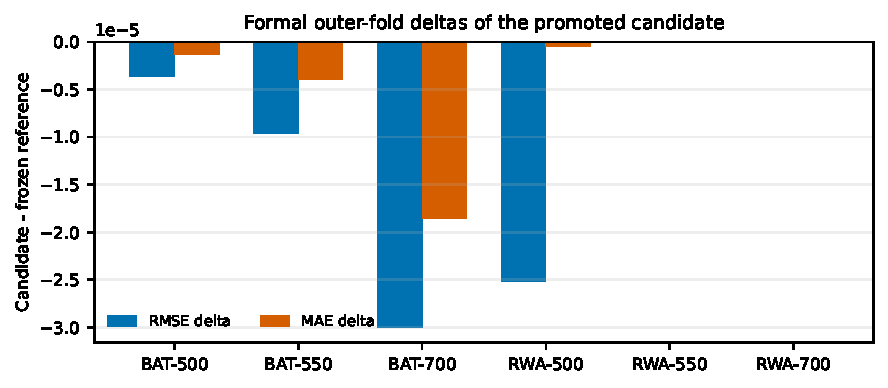
\includegraphics[width=\linewidth]{../figures/formal_deltas.pdf}
\caption{相对冻结参考的形式化差值。零线是晋级阈值。}
\label{fig:deltas}
\end{figure}

\begin{figure}[t]
\centering
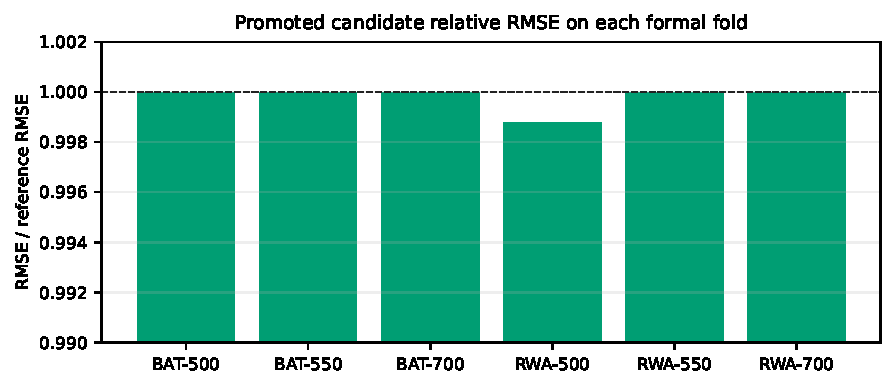
\includegraphics[width=\linewidth]{../figures/relative_rmse.pdf}
\caption{候选与参考的 RMSE 比值。所有晋级折的比值均不大于一。}
\label{fig:ratios}
\end{figure}

\section{审计与可复现性}
最终 receipt 记录六个完整方向、三个残差 KS 对、仅源域路线选择以及恰好一次的外层评估。其 provenance 字段明确记录：canonical 数据未修改；竞赛线未修改；未读取 sealed holdout；未读取 A1/B1 source-heldout；holdout 未用于训练或选择；外层测试未用于选择；总体泛化未验证。最终 receipt 与所有失败 receipt 均保存在隔离研究输出树中。冻结参考和输入张量哈希包含在证据包内。复现需要项目中已经存在的 ModelScope 数据、隔离 runner、固定随机种子以及 receipt 元数据中记录的命令。

\section{局限与适用范围}
形式化结果覆盖三个登记轨道和精确的数据契约，不代表未登记运行工况、未来任务或任意传感器容器上的性能。alpha 下限是从有限目录中仅用源域选择的工程约束，不是学习得到的域不变表示，也不构成一般定理。比较对象是一个冻结的分段 HGB/MLP 参考，因此不能解读为相对于所有 RUL 方法的普遍排名。接近 $10^{-8}$ 的微小差值说明冻结实现、聚合约定和数值容差必须版本化。最后，研究按设计没有读取 sealed、A1 或 B1 holdout，因此总体范围泛化仍未被验证。

\section{结论}
当时序表示、源域拟合修正和 alpha 路线被视为一个版本化协议时，可审计的仅源域路线能够通过严格的六折晋级门禁。最终的 unit-first 残差中心化 TCN 配合统一 $10^{-5}$ alpha 下限，在登记的 BAT/RWA 六个外层折上同时改善 RMSE 和 MAE。本文的主要科学价值在于明确区分源域诊断和外层确认：失败候选被完整保留，最终结论严格限定在受控的未见轨道实验内。

\begin{thebibliography}{00}
\bibitem{bai2018tcn} S. Bai, J. Z. Kolter, and V. Koltun, ``An empirical evaluation of generic convolutional and recurrent networks for sequence modeling,'' arXiv:1803.01271, 2018.
\bibitem{huber1964} P. J. Huber, ``Robust estimation of a location parameter,'' \emph{The Annals of Mathematical Statistics}, vol. 35, no. 1, pp. 73--101, 1964, doi: 10.1214/aoms/1177703732.
\bibitem{ben2010domain} S. Ben-David, J. Blitzer, K. Crammer, A. Kulesza, F. Pereira, and J. W. Vaughan, ``A theory of learning from different domains,'' \emph{Machine Learning}, vol. 79, pp. 151--175, 2010, doi: 10.1007/s10994-009-5152-4.
\bibitem{fawaz2019review} H. I. Fawaz, G. Forestier, J. Weber, L. Idoumghar, and P.-A. Muller, ``Deep learning for time series classification: a review,'' \emph{Data Mining and Knowledge Discovery}, vol. 33, pp. 917--963, 2019, doi: 10.1007/s10618-019-00619-1.
\bibitem{paszke2019pytorch} A. Paszke et al., ``PyTorch: An imperative style, high-performance deep learning library,'' in \emph{Advances in Neural Information Processing Systems}, vol. 32, 2019.
\end{thebibliography}
\end{document}
